\documentclass[border=3mm]{standalone}

\usepackage{tikz}
\usetikzlibrary{decorations.markings,arrows.meta}

\begin{document}
	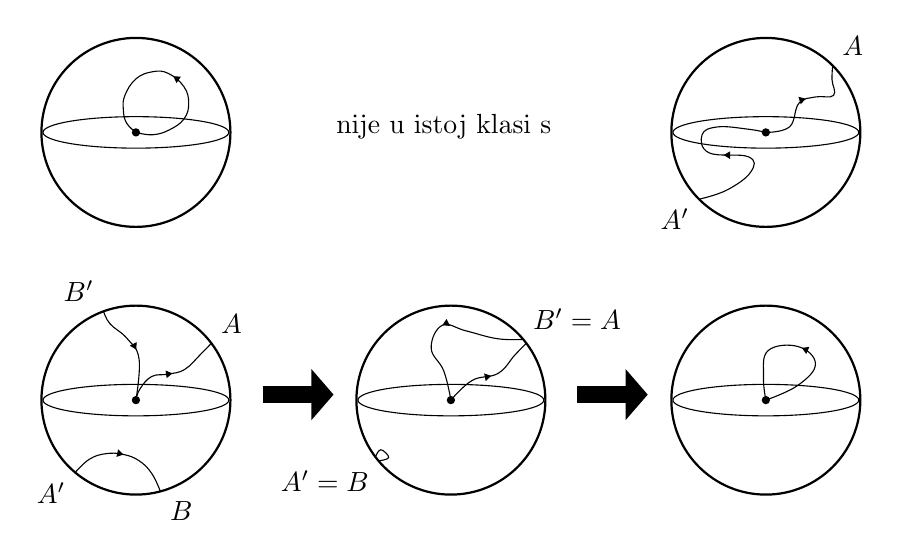
\begin{tikzpicture}
		\begin{scope}[decoration={
			markings,
			mark=at position 0.5 with {\arrow{Triangle[scale=0.65]}}
		}]
			\draw[thick] (-3.91,1.83) coordinate (o1) circle (1.2);
			\draw (o1) ellipse (1.18 and 0.2);
			\draw[postaction={decorate}]  plot[smooth, tension=.7] coordinates {(o1) (-3.7,1.8) (-3.49,1.86) (-3.3,2) (-3.24,2.2) (-3.3,2.41) (-3.5,2.58) (-3.7,2.6) (-3.91,2.51) (-4.05,2.3) (-4.07,2.12) (-4.03,1.95) (o1)};
			\fill (o1) circle (1.5pt);
		\end{scope}
		\begin{scope}[xshift=8cm,decoration={
			markings,
			mark=at position 0.5 with {\arrow{Triangle[scale=0.65]}}
		}]
			\draw[thick] (-3.91,1.83) coordinate (o2) circle (1.2);
			\draw  (o2) ellipse (1.18 and 0.2);
			\path (o2) --++ (45:1.2) coordinate (1) node[above right]{$A$};
			\path (o2) --++ (225:1.2) coordinate (2) node[below left]{$A'$};
			\fill (o2) circle (1.5pt);
			\draw[postaction={decorate}]  plot[smooth, tension=.7] coordinates {(2) (-4.4,1.1) (-4.1,1.33) (-4.13,1.52) (-4.63,1.57) (-4.72,1.8) (-4.52,1.9) (-4.13,1.87) (o2)};
			\draw[postaction={decorate}]  plot[smooth, tension=.7] coordinates {(o2) (-3.61,1.9) (-3.49,2.2) (-3.28,2.28) (-3.05,2.3) (-3.07,2.5) (1)};
		\end{scope}
		\begin{scope}[yshift=-3.4cm,decoration={
			markings,
			mark=at position 0.5 with {\arrow{Triangle[scale=0.65]}}
		}]
			\draw[thick] (-3.91,1.83) coordinate (o3) circle (1.2);
			\draw (o3) ellipse (1.18 and 0.2);
			\path (o3) --++ (37:1.2) coordinate (3) node[above right]{$A$};
			\path (o3) --++ (230:1.2) coordinate (4) node[below left]{$A'$};
			\path (o3) --++ (110:1.2) coordinate (5) node[above left]{$B'$};
			\path (o3) --++ (285:1.2) coordinate (6) node[below right]{$B$};
			\fill (o3) circle (1.5pt);
			\draw[postaction={decorate}]  plot[smooth, tension=.7] coordinates {(4) (-4.5,1.08) (-4.29,1.15) (-4.07,1.14) (-3.87,1.06) (-3.71,0.9) (6)};
			\draw[postaction={decorate}]  plot[smooth, tension=.7] coordinates {(5) (-4.24,2.8) (-4.02,2.61) (-3.87,2.35) (o3)};
			\draw[postaction={decorate}]  plot[smooth, tension=.7] coordinates {(o3) (-3.86,1.97) (-3.71,2.13) (-3.5,2.16) (-3.29,2.22) (-3.09,2.41) (3)};
		\end{scope}
		\begin{scope}[
			xshift=4cm,
			yshift=-3.4cm,
			decoration={
				markings,
				mark=at position 0.5 with {\arrow{Triangle[scale=0.65]}}
			}
		]
			\draw[thick] (-3.91,1.83) coordinate (o4) circle (1.2);
			\draw  (o4) ellipse (1.18 and 0.2);
			\path (o4) --++ (37:1.2) coordinate (7);
			\path (o4) --++ (40:1.2) coordinate (8) node[above right]{$B'=A$};
			\path (o4) --++ (217:1.2) coordinate (9);
			\path (o4) --++ (220:1.2) coordinate (10) node[below left]{$A'=B$};
			\fill (o4) circle (1.5pt);
			\draw[postaction={decorate}] plot[smooth, tension=.7] coordinates {(o4) (-3.64,2.08) (-3.31,2.17) (-3.1,2.4) (7)};
			\draw[postaction={decorate}] plot[smooth, tension=.7] coordinates {(8) (-3.32,2.61) (-3.72,2.71) (-4.02,2.78) (-4.16,2.49) (-4,2.2) (o4)};
			\draw  plot[smooth, tension=.7] coordinates {(10) (-4.7,1.1) (-4.8,1.2) (9)};
		\end{scope}
		\begin{scope}[
			xshift=8cm,
			yshift=-3.4cm,
			decoration={
				markings,
				mark=at position 0.5 with {\arrow{Triangle[scale=0.65]}}
			}
		]
			\draw[thick] (-3.91,1.83) coordinate (o5) circle (1.2);
			\draw  (o5) ellipse (1.18 and 0.2);
			\draw[postaction={decorate}]  plot[smooth, tension=.7] coordinates {(o5)  (-3.5,2.02)  (-3.28,2.29)  (-3.5,2.51)  (-3.88,2.46)  (-3.94,2.13)  (o5)};
			\fill (o5) circle (1.5pt);
		\end{scope}
		\node at (0,1.9) {nije u istoj klasi s};
		\draw[-{Triangle[width=18pt,length=8pt]}, line width=6pt] (-2.3,-1.5) -- (-1.4,-1.5);
		\draw[-{Triangle[width=18pt,length=8pt]}, line width=6pt] (1.69,-1.5) -- (2.59,-1.5);
	\end{tikzpicture}
\end{document}